\subsection{阶段的优化与分析}
\subsubsection{combiner阶段}
Google提出的MapReduce中,在map阶段加入了可选的combiner操作,所谓combiner就是局部的reduce操作,将一个key对应的多个value进行局部的归并,这样可以有小减少网路通信量,以及本地磁盘空间的使用。多核环境下的combiner思想与分布式环境下的combiner一致,但其主要作用不是减少网络通信量,而是降低时间和空间的开销。

采用array buffer时,
开启combiner的优势是:
可以减少物理内存的使用(物理映射,通道需传输的数据量)。
但开启Map阶段的combiner带来的开销有两部分:
回调combiner函数的开销、
对key排序的开销。
最终的结果如图\ref{dmr:combiner}
\begin{figure}[!h!t]  
    \centering
    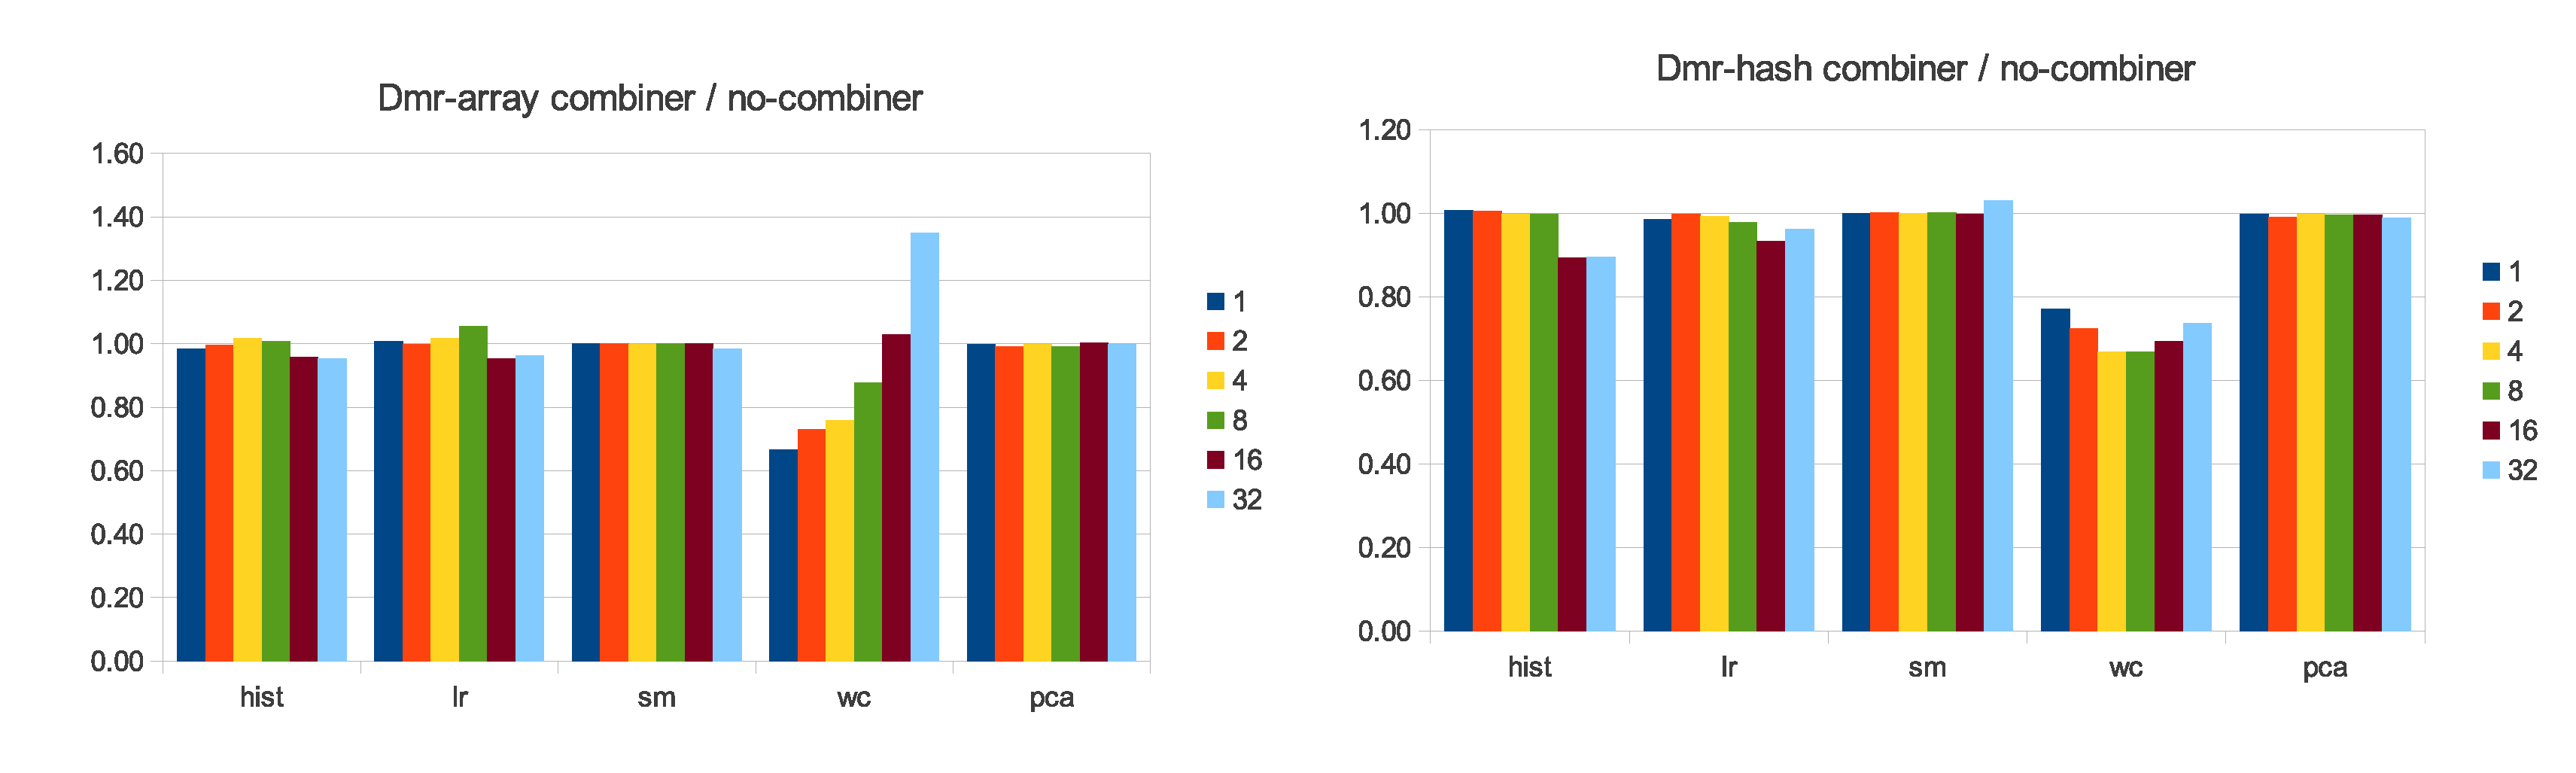
\includegraphics[width=1\textwidth]{img/dmr_combiner.eps}
    \caption{combiner or No-combiner}
    \label{dmr:combiner}
\end{figure}

总结:如果Map阶段开启combiner,
为了给key排序,其时间复杂度为O(n).
是否开启combiner与应用程序有关
\begin{itemize}
  \item 如果应用程序的重复的key较多,
  那么map阶段开启combiner较好,
  可减少内存重映射的开销,
  又由于不同key的数量较少,
  array的查找长度较短,从而开启combiner具有较好的效果。
  如hist,wc,lr
  
  \item 如果应用程序中重复的key并不多,
  那么开启combiner并不能带来优势,
  如sm,pca
\end{itemize}



\subsubsection{merge阶段}
DMR库中merge阶段的任务类型分三类情况:
\begin{itemize}
  \item 应用程序有map阶段,也有reduce阶段;这种情况下,merge阶段将reduce产生的局部结果进行二路归并,并将最终结果发送给master。这类应用程序包括:histogram, word\_count,linear\_regression, kmeans
  \item 应用程序只有map阶段,没有reduce阶段;此时,map阶段产生键值对,即为结果数据,该键值对将被直接发送给merge,merge对这些局部数据进行二路归并,最终结果发送给master。这类应用程序包括pca,matrix\_multiply
  \item 应用程序只有map阶段,且map阶段不产生键值对。该情况下,是不需要进行merge过程的;这类应用程序包括string\_match
\end{itemize}

MapReduce处理流程中的reduce阶段中的每个reduce线程最终会产生一个全局的结果,但该结果只是整个结果的一些片段。为了得到完成的结果数据,需要经过merge阶段的数据汇集。因此merge阶段的主要任务是汇集多个局部结果,将其归并为一个最终的完整结果,并将结果发送给master线程。

DMR中merge阶段采用二路归并的方式,将各个reduce线程的局部结果,归并为一个完整的数据

\begin{figure}[!h]
    \centering
    \includegraphics[height=4cm,width=6cm]{img/merge_opt.png}
    \caption{merge optimize}
\label{merge_opt}
\end{figure}
针对string\_match,经过merge阶段的优化之后,性能对比如图\ref{merge_opt}
